\title{Android -- Eine Einführung}
\subtitle{Entwicklungsumgebung, Aufbau, Komponenten \& Widgets}
\author[A. Wilhelm]{Andreas Wilhelm}
\institute[www.avedo.net]{}
\titlegraphic{}
%\date{\today}
\date{CSC Computer-Schulung \& Consulting GmbH}

\begin{frame}[plain]
  \titlepage
\end{frame}

\section[Contents]{}
\begin{frame}
	\frametitle{Contents}
	\tableofcontents[onlyparts]
\end{frame}

% 1 Die Entwicklungsumgebung
% 1.1 Android SDK
% 1.2 Eclipse
% 1.3 Das ADT Plugin
% 1.4 Der Emulator
\part{Eclipse \& Android SDK}
\frame{\partpage}
\begin{frame}
	\frametitle{Contents}
	\tableofcontents[]
\end{frame}

\section{Eclipse \& Android}
\begin{frame}[label=eclipse_sdk]
   \frametitle{Eclipse \& Android}
   \begin{itemize}
      \item Gemeinsame Oberfläche für verschiedene Entwicklungstools
      \item Basis für Android-Entwicklung -- Android Software Development Kit (SDK)
      \item \href{http://developer.android.com/sdk/}{http://developer.android.com/sdk/}
      \item Einbindung in Eclipse über das ADT-Plugin
      \item \href{http://developer.android.com/tools/sdk/eclipse-adt.html}{http://developer.android.com/tools/sdk/eclipse-adt.html}
   \end{itemize}
\end{frame}

\section{Das Android SDK}
\begin{frame}[label=eclipse_adt]
   \frametitle{Das Android SDK}
   \begin{itemize}
      \item Stellt Bibliotheken zur Android-Entwicklung zur Verfügung
      \item Zusätzliche Entwicklertools zum Testen \& Debuggen
      \item Standard Support Library für Abwärtskompatibilität
      \item Ausführliche Anwendungsbeispiele
      \item Installer für Windows \& Linux 32-bit verfügbar
      \item Unter Linux 64-bit muss \emph{ia32-libs} Paket installiert werden
   \end{itemize}
\end{frame}

\section{Der Emulator}
\begin{frame}[label=emulator]
   \frametitle{Der Emulator}
   \begin{itemize}
      \item Simulation der Applikation unter verschiedenen Android Versionen
      \item Testen der Applikation bei verschiedenen Auflösungen
      \item Konfiguration verschiedener Geräte-Typen (Motorrola, HTC, ...)
      \item Verwalten verschiedener Konfigurationen über den 
         Android-Virtuell-Device-(AVD)-Manager
      \item Automatisches Kompilieren, Uploaden und Starten der Applikation 
         auf dem Emulator aus Eclipse heraus
   \end{itemize}
\end{frame}

% 2 Aufbau einer Applikation
% 2.1 Das Manifest
% 2.2 Resourcen
% 2.3 Aktivitäten und Layouts
\part{Aufbau einer Applikation}
\frame{\partpage}
\begin{frame}
	\frametitle{Contents}
	\tableofcontents[]
\end{frame}

\section{Das Android Manifest}
\begin{frame}[label=manifest]
   \frametitle{Eigenschaften}
   Enthält grundlegende Informationen über eine Applikation wie
   \begin{itemize}
      \item Name, Paketname und Version der Applikation
      \item Verwendete Komponenten (Aktivitäten, Services und Broadcast Receiver)
      \item Zugangsmöglichkeiten zu den einzelnen Komponenten (Broadcasts, ...)
      \item Zugriffsrechte der Applikation (Internet, Anrufe, ...)
      \item Benötigte Zugriffsrechte anderer Applikationen zur Verwendung 
         von Komponenten dieser Applikation
      \item Minimal und Maximal unterstützte API-Version
      \item Definition in Form einer eXtended-Markup-Language(XML)-Datei
   \end{itemize}
\end{frame}

\begin{frame}[fragile, label=manifest_structure]
   \frametitle{Bispiel}
   \lstinputlisting[language=xml,label={lst:manifest.xml},
		caption={Beispielstruktur einer Manifest-Datei}]{src/xml/manifest.xml}
\end{frame}

\section{Ressourcenverwaltung}
\begin{frame}[label=resources]
   \frametitle{Überblick}
   \begin{itemize}
      \item Trennung von Quellcode und Resourcen (Bildern, Zeichenketten, Layouts, ...)
      \item Eröffnet Möglichkeit verschiedenste Geräte zu unterstützen
      \item Verwaltung der Resourcen in Verzeichnisstruktur unter \emph{res}
      \item Feste Konventionen zur Einsortierung von Resourcen 
         (Beispiel: \emph{res/values/strings.xml} und \emph{res/values-de/strings.xml})
      \item Zugriff auf Resourcen aus dem Quellcode über automatisch generierte Klasse \emph{R}
      \item Referenzierung der Resourcen über IDs (Beispiel: \emph{R.string.btnOk})
   \end{itemize}

   \lstinputlisting[language=xml,label={lst:strings.xml},
      caption={String Resourcen}]{src/xml/strings.xml}
\end{frame}

\begin{frame}[label=resources]
   \frametitle{Beispiele}

   \lstinputlisting[language=xml,label={lst:colors.xml},
      caption={Farb Resourcen}]{src/xml/colors.xml}
   
   \lstinputlisting[label={lst:resources.java},
   	caption={Zugriff auf Resourcen}]{src/java/resources.java}
\end{frame}

% 3 Komponenten in Android
% 3.1 Aktivitäten
% 3.2 Fragmente
% 3.3 Views und View-Groups
% 3.4 Intents
% 3.4.1 Explizite Intents
% 3.4.2 Implizite Intents
% 3.4.3 Ergebnisse von Intents
% 3.4.4 Intent-Filter
% 3.4.5 PendingIntents
% 3.5 Services
% 3.6 Content-Provider
% 3.7 Broadcast-Receiver
\part{Komponenten in Android}
\frame{\partpage}
\begin{frame}
	\frametitle{Contents}
	\tableofcontents[]
\end{frame}

\section{Aktivitäten}
\begin{frame}[label=activities]
   \frametitle{Allgemeines}
   \begin{itemize}
      \item Aktivitäten (Activities) bilden die Präsentationsschicht einer Applikation
      \item Eine Applikation kann aus mehreren Aktivitäten (Dialoge oder Seiten) bestehen
      \item Implementierung einer Aktivität durch Ableitung einer Kindklasse von \emph{Activity}
      \item Wichtig: Überschreiben der Methode \emph{onCreate(Bundle)}
      \item Zuweisung der grafischen Oberfläche mittels der Methode \emph{setContentView(View)}
   \end{itemize}

   \lstinputlisting[label={lst:activity.java},
   	caption={Basisimplementation einer Aktivität}]{src/java/activity.java}
\end{frame}

\begin{frame}[label=activities_states]
   \frametitle{Lebenszyklus}
   Neben \emph{onCreate()} gibt es weitere Callback-Methoden, die auf 
   Zustandsänderungen der Aktivität reagieren. Man spricht vom \emph{Activity Lifecycle}.\\

   Aus der Stack basierten Struktur des Systems ergeben sich folgende Zustände 
   für eine Aktivität:

   \begin{description}
      \item[Running] Aktuell im Vordergrund befindliche Aktivität
      \item[Paused] Sichtbare, aber nicht mehr im Fokus befindliche Aktivität --
         Aktivität bleibt aktiv und der WindowManager hat weiterhin Zugriff -- 
         Aktivität kann trotzdem bei Resourcenmangel vom System beendet werden
      \item[Stopped] Nicht sichtbare Aktivitäten -- alle Einstellungen und 
         Zustände gespeichert -- werden häufig vom System beendet
      \item[Finished] Vom System beendete Aktivität -- muss neu gestartet 
         werden und die Einstellungen der letzten Sitzung neu geladen werden, 
         falls sie erneut den Fokus bekommt
   \end{description}
\end{frame}

\begin{frame}[label=activities_lifecycle]
   \frametitle{Ablaufdiagramm}
   \begin{figure}[h!]
     \centering
     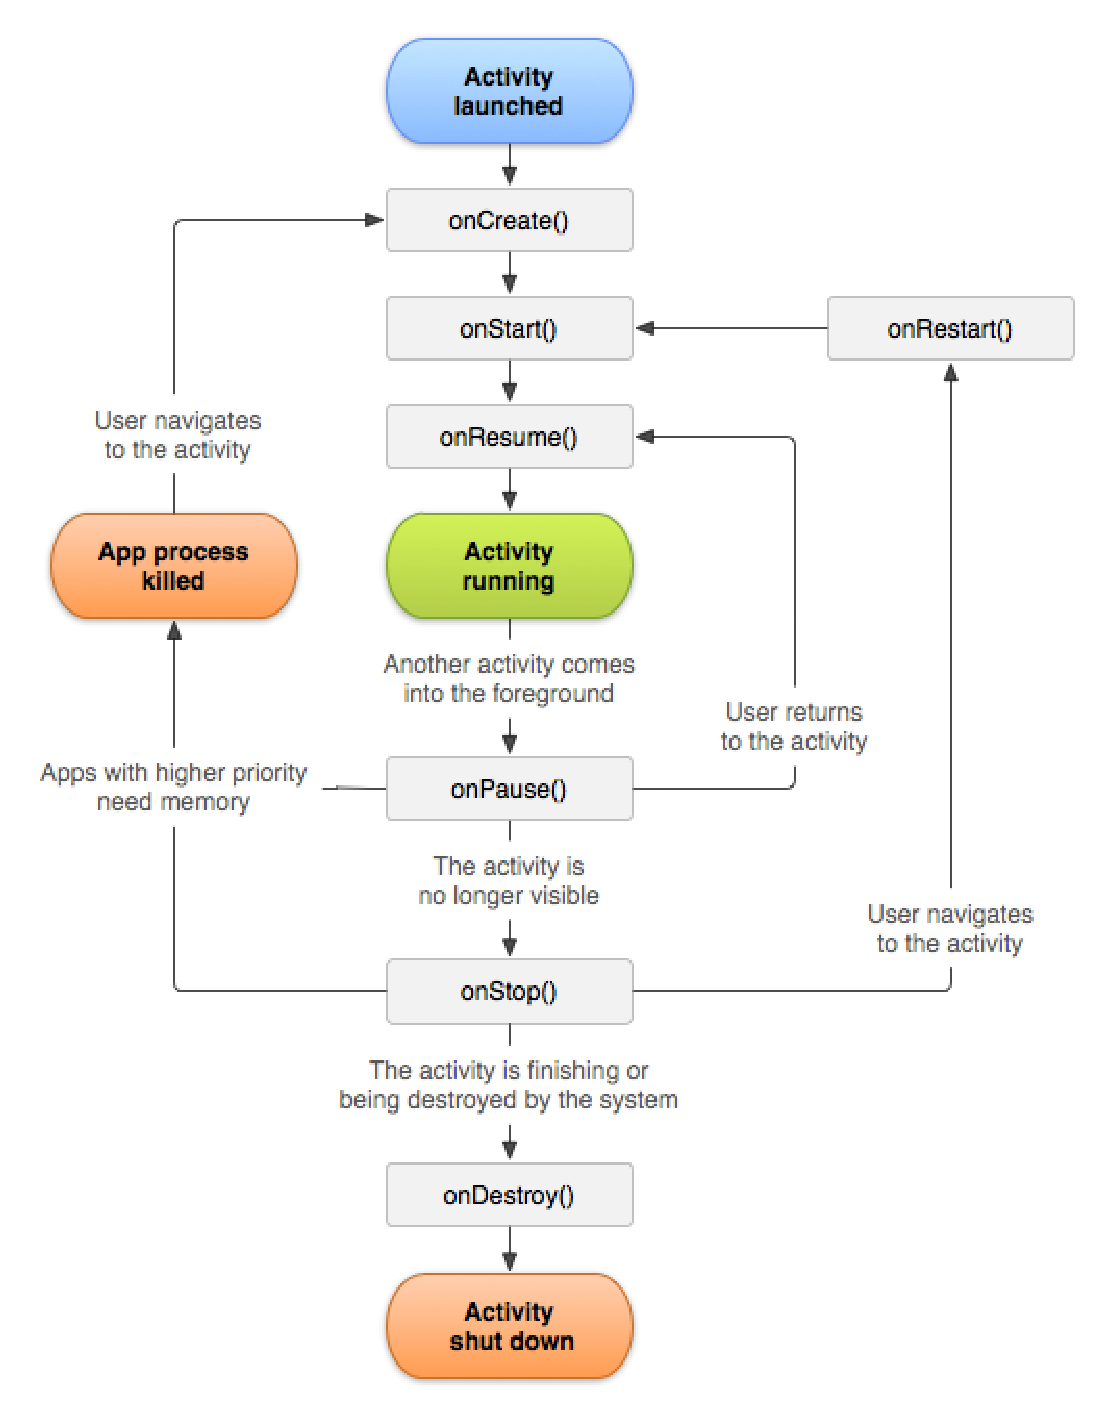
\includegraphics[width=0.45\textwidth]{pictures/activity_lifecycle.eps}
     \caption{
        Der Aktivity Lifecycle 
        (\emph{Quelle: 
           \href{http://developer.android.com}{http://developer.android.com}})
     }
     \label{fig:activity_lifecycle}
   \end{figure}
\end{frame}

\section{Fragmente}
\begin{frame}[label=fragments]
   \frametitle{Allgemeines}
   \begin{itemize}
      \item Teil einer Aktivität -- Eine Aktivität kann meherere Fragments enthalten
      \item Eingeführt in Android Version 3.0 (API-Version 11)
      \item Flexiblere grafische Oberflächen für größere Displays
      \item Einfacheres Austauschen und Wiederverwerten von Teilen der Oberfläche
      \item Verhalten ähnlich einer Aktivität -- Lebenszyklen eng verbunden\\
      	$\rightarrow$ Sollte Aktivität beendet werden, werden alle beinhalteten 
      		Fragmente beendet
   \end{itemize}
   
   Zustände eines Fragments ähneln denen einer Aktivität:

	\begin{description}
		\item[Laufend] Das Fragment ist sichtbar innerhalb der aktiven Aktivität. 
		\item[Pausiert] Die beinhaltende Aktivität ist zwar zumindest teilweise sichtbar, 
			läuft aber im Hintergrund.
		\item[Gestoppt] Entweder die beinhaltende Aktivität wurde beendet oder 
			das Fragment wurde entfernt und auf dem ''Zurück''-Stapel (\emph{Backstack})
			der Aktivität abgelegt. Das Fragment ist jedoch, auch wenn nicht sichtbar, 
			immernoch aktiv.
	\end{description}
\end{frame}

\begin{frame}[label=fragments]
   \frametitle{Lebenszyklus}
   
   \begin{alertblock}{Backstack}
		Android unterscheidet zwischen System- und Aktivitäten-Backstack. Aktivitäten 
		werden automatisch auf den System-Backstack, Fragmente nur nach expliziter 
		Aufforderung auf Aktivitäten-Backstack abgelegt. 
   \end{alertblock}
   
   Neben von Aktivitäten bekannten Methoden, wie \emph{onCreate()}, \emph{onPause()} 
	und \emph{onResume()} implementieren Fragmente weitere Methoden zur Synchronisation:

	\begin{description}
		\item[onAttach()] Fragment wird mit Aktivität assoziiert
		\item[onCreateView()] Layout des Fragments soll erstellt bzw. geladen werden
		\item[onActivityCreated()] Aufruf der Methode \emph{onCreate()} der Aktivität wurde beendet
		\item[onDestroyView()] Ansicht wird aufgelöst
		\item[onDetach()] Assoziation zwischen Fragment und Aktivität wurde aufgehoben
	\end{description}
\end{frame}

\begin{frame}[label=activity_fragment_lifecycle]
   \frametitle{Ablaufdiagramm}
	\begin{figure}[h!]
	  \centering
	  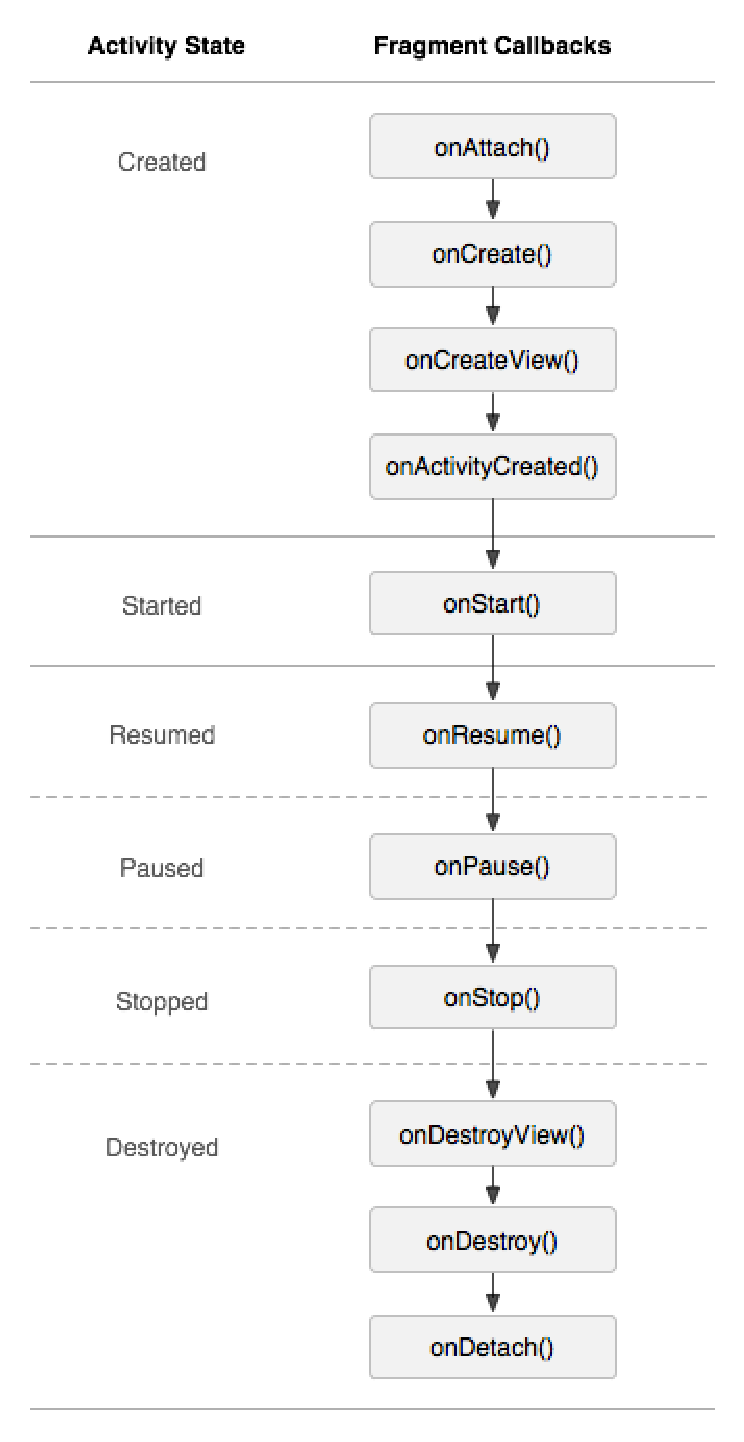
\includegraphics[width=0.3\textwidth]{pictures/activity_fragment_lifecycle.eps}
	  \caption{
		  Der Lebenszyklus eines Fragments
		  (\emph{Quelle: 
		     \href{http://developer.android.com}{http://developer.android.com}})
	  }
	  \label{fig:activity_fragment_lifecycle}
	\end{figure}
\end{frame}

\begin{frame}[label=fragment_implementation]
   \frametitle{Implementierung}
   \begin{itemize}
      \item Ableiten einer eigenen Klasse von \emph{Fragment}, \emph{ListFragment}, 
      	\emph{PreferenceFragment} oder \emph{WebViewFragment}
      \item Implementiert werden sollten \emph{onCreate()}, 
			\emph{onCreateView()} und \emph{onPause()}
      \item Wichtig: Änderungen sollten in \emph{onPause()} gespeichert werden, 
      	denn es ist nicht sicher ob Benutzer zurückkehrt
      \item Einbettung des Fragments in Layout der Aktivität über 
      	\emph{\textless{}fragment\textgreater}
      \item Alternativ Integration über Vater-ViewGroup des Fragments 
      	im Quellcode
   \end{itemize}

   \begin{alertblock}{IDs und Tags}
		Fragments sollten bei ihrer Integration mit \emph{\textless{}fragment\textgreater} 
		eine ID zugewiesen bekommen. Dies kann über die XML-Attribute \emph{android:id} oder 
		\emph{android:tag} geschehen, aber auch automatisch durch Zuweisung zu einer ViewGroup, 
		wobei die ID der ViewGroup verwendet wird.\\
   \end{alertblock}
   
   \begin{alertblock}{Umrüstung}
		Die großen Ähnlichkeiten im Aufbau von Fragmenten und Aktivitäten, macht es 
		zumeist sehr einfach eine Applikation auf Fragmente umzurüsten. 
		Oftmals reicht es den Quellcode aus einer Methode der Aktivität in die 
		entsprechende Methode des Fragments zu verschieben.
   \end{alertblock}
\end{frame}

\begin{frame}[label=first_fragment]
   \frametitle{Ein Fragment}
	\lstinputlisting[caption=Das erste Fragment,
		label={lst:OverviewFragment.java}]{src/java/OverviewFragment.java}
\end{frame}

\begin{frame}[label=include_layout_fragment]
   \frametitle{Ein Fragment}
	\lstinputlisting[
		language=xml,caption=Einbinden des Fragments,label={lst:large_release_list.xml}]
		{src/xml/large_release_list.xml}
\end{frame}

\begin{frame}[label=fragment_transactions]
   \frametitle{Transaktionen}
   \begin{itemize}
      \item Hinzufügen, Ersetzen und Löschen von Fragments in Aktivität
      \item Verarbeitung von \emph{FragmentTransaction} mit \emph{FragmentManager}
      \item Aktivitäten-Backstack verwaltet Fragment-Transaktionen
      \item Einbinden des Fragments in Layout der Aktivität über \emph{\textless{}fragment\textgreater}
      \item Alternativ Integration über Vater-ViewGroup des Fragments
      \item Mehrere Fragments zu Navigationszwecken
      \item Problem: Unterscheidung für große und kleine Displays nötig
   \end{itemize}
\end{frame}

\begin{frame}[label=fragment_transactions]
   \frametitle{Transaktionen im Einsatz}
	\lstinputlisting[caption=Eine FragmentTransaction,
		label={lst:fragmentTransaction.java}]{src/java/fragmentTransaction.java}
\end{frame}

\begin{frame}[label=activity_layout]
   \frametitle{Aktivitäten-Lösung}
	\begin{figure}[h!]
	  \centering
	  \subfigure[Erste Aktivität mit Liste]{
		  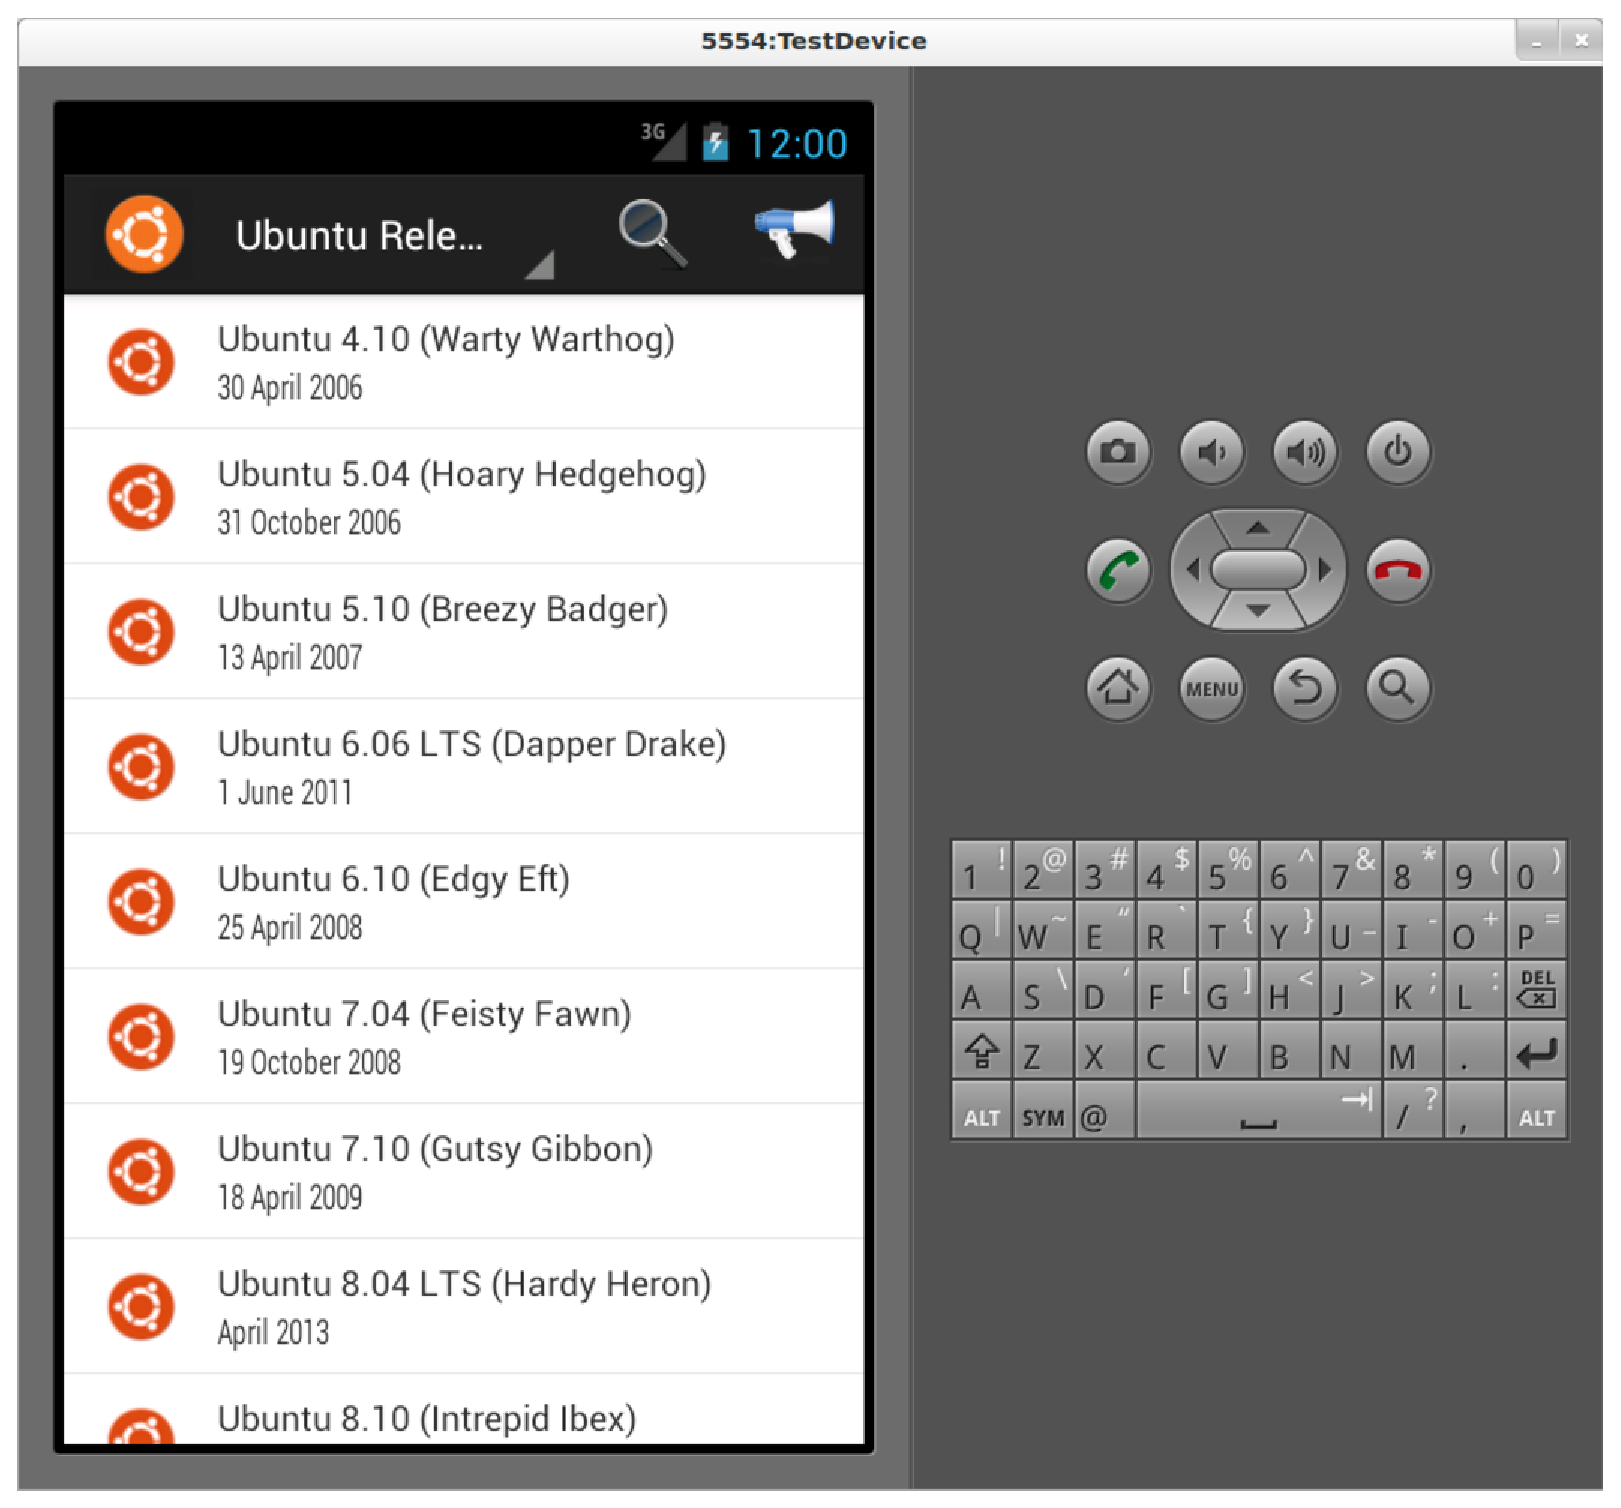
\includegraphics[width=0.47\textwidth]{pictures/ubuntu_list_rows.eps}
		  \label{fig:ubuntu_list_rows}
	  }\hfill
	  \subfigure[Zweite Aktivität mit Zusatzinformationen]{
		  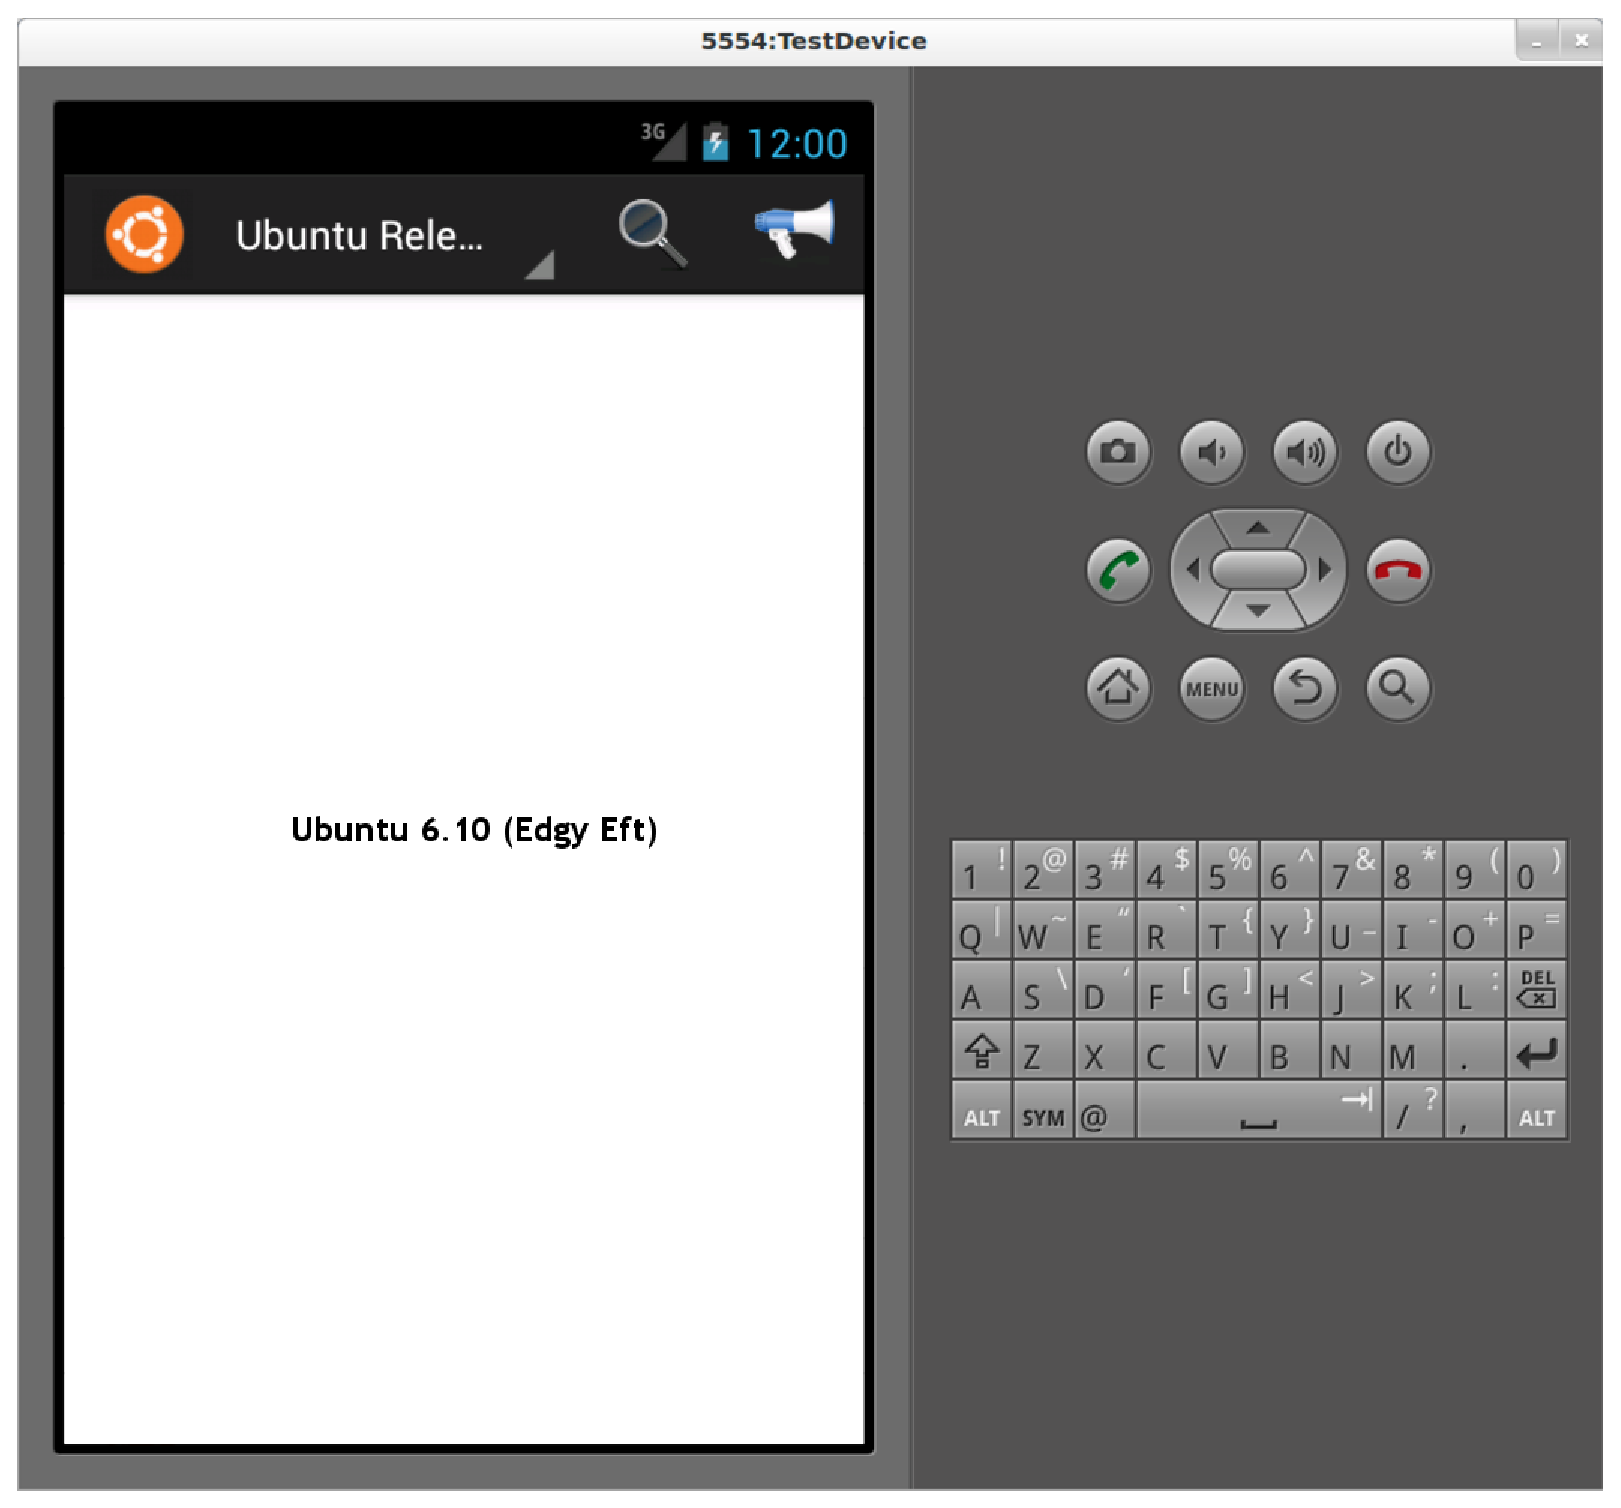
\includegraphics[width=0.47\textwidth]{pictures/ubuntu_list_rows_empty.eps}
		  \label{fig:ubuntu_list_rows_empty}
	  }
	  \caption{
		  Navigation mit zwei Aktivitäten
	  }
	  \label{fig:ubuntu_activity_list}
	\end{figure}
\end{frame}

\begin{frame}[label=fragment_layout]
   \frametitle{Fragment-Lösung}
	\begin{figure}[h!]
	  \centering
	  \includegraphics[width=0.9\textwidth]{pictures/ubuntu_list_large.ps}
	  \caption{
		  Navigation mit zwei Fragments
	  }
	  \label{fig:ubuntu_fragment_list}
	\end{figure}
\end{frame}

\begin{frame}[label=fragments_without_layout]
   \frametitle{Fragments ohne Layout}
   \begin{itemize}
      \item Fragmente ohne Layout als Erweiterungen von Aktivitäten
      \item Implementierung von Hintergrundarbeiten
      \item Implementierung von oft verwendeten Menüs
      \item Zuweisung von Fragmenten ohne Layout mit \emph{add()}
      \item Laden dieser Fragments mit \emph{findFragmentByTag()}
      \item \emph{onCreateView()} wird nicht aufgerufen
   \end{itemize}
\end{frame}

\section{Views und View-Groups}
\begin{frame}[label=views]
   \frametitle{Allgemeines}
   \begin{itemize}
      \item Teile von Benutzeroberflächen, wie beispielsweise Buttons, Auswahl- 
         oder Texteingabefelder
      \item Definition in Form einer XML-Datei
      \item Aussehen und Verhalten kann über XML-Attribute verändert werden
      \item \emph{ViewGroups} (auch LayoutManager) dienen zur Strukturierung und Anordung 
         von Views
      \item Eine beliebige Verschachtelung von ViewGroups ist möglich
   \end{itemize}
\end{frame}

\begin{frame}[label=access_views]
   \frametitle{Beispiel}

   \lstinputlisting[language=xml,caption={Ein einfaches Layout},
		label={lst:view.xml}]{src/xml/view.xml}
\end{frame}

\begin{frame}[label=access_views]
   \frametitle{Zugriff im Quellcode}
   \begin{itemize}
      \item Zugriff auf Views und ViewGroups aus dem Quellcode heraus über \emph{findViewById()}
      \item Laden eines Layouts ohne Verwendung von \emph{setContentView()} mit \emph{LayoutInflater}
   \end{itemize}

   \lstinputlisting[label={lst:access_view.java},
		caption={Zugriff auf das Layout}]{src/java/access_view.java}
\end{frame}

\section{Intents}
\begin{frame}[label=intents]
   \frametitle{Überblick}
   \begin{itemize}
      \item Nachrichten zur Kommunikation innerhalb des Systems
      \item Aufruf von Funktionalitäten des Systems
      \item Übertragung von Daten zwischen verschiedenen Komponenten
      \item Methoden \emph{startActivity} und \emph{startService}, sowie 
         \emph{sendBroadcast} nutzen Intents
      \item Unterscheidung zwischen expliziten und impliziten Intents
   \end{itemize}
\end{frame}

\begin{frame}[label=explizit_intents]
   \frametitle{Explizite Intents}
   Der Empfänger der Nachricht wird explizit angegeben.

   \lstinputlisting[caption={Starten einer Aktivität},
		label={lst:explicit_intent.java}]{src/java/explicit_intent.java}
   
   Die übertragenden Daten können in der \emph{onCreate()} Methode extrahiert 
   und verarbeitet werden.

   \lstinputlisting[caption={Extrahieren der Daten},
		label={lst:explicit_intent_extract.java}]{src/java/explicit_intent_extract.java}
\end{frame}

\begin{frame}[label=implizit_intents]
   \frametitle{Implizite Intents}
   Anders als bei expliziten Intents, wird bei der Verwendung impliziter Intents 
   nicht spezifiziert welche Komponente verwendet werden soll.

   \lstinputlisting[caption={Auswahl der Komponente},
   	label={lst:implicit_intent.java}]{src/java/implicit_intent.java}
   
   \begin{itemize}
      \item System kann die richtige Komponente für die gegebene Aktion auswählen
      \item Man kann dem Benutzer die Möglichkeit geben eine andere Applikation zu nutzen
      \item Es kann auf andere Applikationen zurückgegriffen werden ohne die
         benötigte Funktionalität selbst zu implementieren
   \end{itemize}
\end{frame}

\begin{frame}
   \frametitle{Ergebnisse von Intents}
   
   \lstinputlisting[caption={Starten der Aktivität},
   	label={lst:start_for_result.java}]{src/java/start_for_result.java}

   \lstinputlisting[caption={Ergebnisse senden},
   	label={lst:result_intent.java}]{src/java/result_intent.java}
\end{frame}

\begin{frame}
   \frametitle{Ergebnisse von Intents}
   \lstinputlisting[caption={Ergebnisse empfangen},
      label={lst:on_activity_result.java}]{src/java/on_activity_result.java}
\end{frame}

\begin{frame}
   \frametitle{Intent-Filter}
   \begin{itemize}
      \item Legen fest auf welche impliziten Intents eine Komponente anspricht
      \item Explizite Intents sind nicht von Filtern betroffen
      \item Ermöglicht Reaktion auf System-Events (ankommende SMS, Systemstart, ...)
   \end{itemize}

   \lstinputlisting[caption={Deklaration im Manifest},
		language=xml,label={lst:intent_filter.xml}]{src/xml/intent_filter.xml}
\end{frame}

\section{Pending Intent}
\begin{frame}
   \frametitle{Allgemeines}
   \begin{itemize}
      \item PendingIntents kapseln ein Intent und die zur Verwendung benötigten Rechte
      \item Delegation von Rechten an andere Applikationen bzw. das System
      \item Starten von Broadcasts und Aktivitäten 
      \item \emph{PendingIntent.getBroadcast()} bzw. \emph{PendingIntent.getActivity()} 
      \item Beispiel: Notification-Manager
   \end{itemize}
\end{frame}

\begin{frame}
   \frametitle{Beispiel}
	\lstinputlisting[caption=Email Benachrichtigung,label={lst:email_notification.java}]{src/java/email_notification.java}
\end{frame}

\section{Services}
\begin{frame}[label=services]
   \frametitle{Allgemeines}
   \begin{itemize}
      \item Im Hintergrund arbeitende Komponenten für länger andauernde Operationen
      \item Bietet keine eigene Oberfläche
      \item Läuft im selben Thread wie die Applikation
      \item Können von einer anderen Komponente, Applikation oder durch ein 
         Event (BroadcastReceiver) gestartet werden
      \item Kann an eine andere Komponente gebunden werden um mit ihr zu interagieren
   \end{itemize}

   Ein Service kann zwei Zustände annehmen:

   \begin{description}
   \item[Gestartet] (Aufruf mit \emph{startService()})
      \begin{itemize}
         \item Beendet sich am Schluss selbst ohne ein Ergebnis zu liefern
         \item Kann praktisch unendlich laufen, auch wenn die startende 
            Komponente beendet wurde
      \end{itemize}  
   \item[Gebunden] (Aufruf mit \emph{bindService()})
      \begin{itemize}
         \item Service wurde von anderen Komponente mit \emph{bindService()} an sich gebunden 
         \item Interaktion (Nachrichten, Ergebnisse und Anfragen) mit startender Komponente möglich
         \item Bindung an beliebig viele Komponenten möglich
         \item Falls alle verbundenen Komponenten beendet oder getrennt werden, 
            wird der Service beendet
      \end{itemize}  
   \end{description}
\end{frame}

\begin{frame}[label=services]
   \frametitle{Beispiel}
   \lstinputlisting[caption={Ein einfacher Service},
   	label={lst:service.java}]{src/java/service.java}
\end{frame}

\section{Content-Provider}
\begin{frame}[label=content_provider]
   \frametitle{Content-Provider}
   \begin{itemize}
      \item Verwalten den Zugriff auf Daten und stellen diese global zur Verfügung
      \item Kapseln die Daten und bieten Mechanismen zum Datenschutz
      \item \emph{ContentResolver} ermöglichen die Kommunikation mit 
         einem \emph{ContentProvider} als Client
      \item ContentProvider werden beötigt, wenn Daten zwischen Applikationen 
         kopiert werden sollen oder angepasste Suchergebnisse benötigt werden
      \item Es existieren Android eigene ContentProvider für Audio, Video, 
         Bilder und Kontakte
   \end{itemize}
\end{frame}

\section{Broadcast-Receiver}
\begin{frame}[label=broadcast_receiver]
   \frametitle{Broadcast-Receiver}
   \begin{itemize}
      \item Empfänger von Intents die mit \emph{sendBroadcast()} versendet wurden
      \item Kommunikation zwischen verschiedenen Komponenten
      \item Reagieren auf System-Events
   \end{itemize}

   \lstinputlisting[caption={Deklaration im Manifest},
   	language=xml,label={lst:broadcast_receiver.xml}]{src/xml/broadcast_receiver.xml}

   \lstinputlisting[caption={Implementierung},
		label={lst:broadcast_receiver.java}]{src/java/broadcast_receiver.java}
\end{frame}

% 4.7 Widgets
% 4.7.1 Das Widget Layout
% 4.7.2 Die AppWidgetProviderInfo
% 4.7.3 Der AppWidgetProvider
\part{Widgets}
\frame{\partpage}
\begin{frame}
	\frametitle{Contents}
	\tableofcontents[]
\end{frame}

\section{Überblick}
\begin{frame}[label=widgets]
   \frametitle{Widgets}
   \begin{itemize}
      \item Miniaturansicht, die in andere Applikationen, wie den Desktop integriert werden können
      \item Widgets werden periodisch aktualisiert
      \item Besteht aus folgenden Komponenten:
         \begin{description}
            \item[AppWidgetProviderInfo] XML-Datei, die für das System wichtige Informationen enthält
            \item[AppWidgetProvider] Implementiert die grundlegenden Methoden 
               um mit dem Widget zu interagieren.
            \item[Widget View] Definiert das zu Anfang sichtbare Layout (XML-Datei)
         \end{description}
   \end{itemize}

   \begin{figure}[h!]
      \centering
      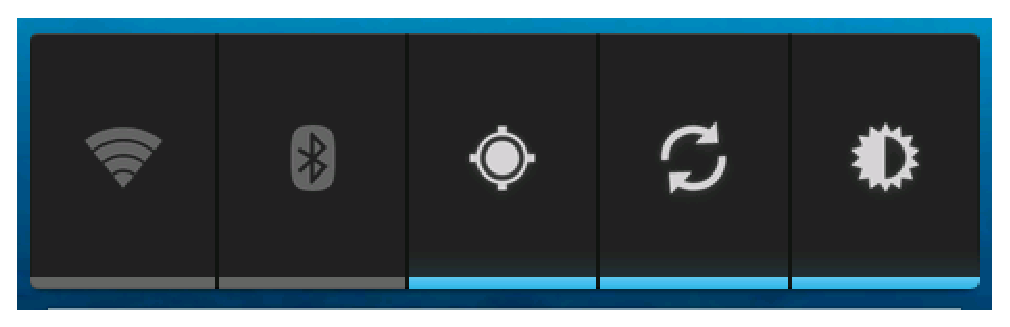
\includegraphics[width=0.5\textwidth]{pictures/widget.eps}
      \caption{Das Einstellungs-Widget}
      \label{fig:widget}
   \end{figure}

   Optional kann auch eine gesonderte Aktivität zur Konfiguration des 
   Widgets hinterlegt werden.
\end{frame}

\section{Widget Layout}
\begin{frame}[label=widget_layout]
   \frametitle{Widget Layout}
   \begin{itemize}
      \item Deklaration des Layouts in Form von XML
      \item Layouts werden in \emph{res/layouts/} gespeichert
      \item Nicht alle Views und ViewGroups können verwendet werden (\emph{NumberPicker})
   \end{itemize}

   \lstinputlisting[caption={Das Widget Layout},language=xml,
   	label={lst:widget_layout.xml}]{src/xml/widget_layout.xml}
\end{frame}

\section{Die AppWidgetProviderInfo}
\begin{frame}[label=widget_provider_info]
   \frametitle{Die AppWidgetProviderInfo}
   \begin{itemize}
      \item Definiert alle essentiellen Rahmenbedingungen eines Widgets
         (initiales Layout, Bemaßungen, Dauer bis zur Aktualisierung)
      \item Deklaration in Form einer XML-Datei
   \end{itemize}

   \lstinputlisting[
   	language=xml,label={lst:app_widget_provider_info.xml},
   	caption={Die Widget Info}]{src/xml/app_widget_provider_info.xml}
   	
   Die Attribute des \emph{appwidget-provider} Elements:
   
   \begin{description}
      \item[minWidth] Minimale Breite des Widgets in \emph{dip}
      \item[minHeight] Minimale Höhe des Widgets in \emph{dip}
      \item[updatePeriodMillis] Dauer bis zur nächsten Aktualisierung 
         des Widgets in Millisekunden
      \item[initialLayout] Das initiale Layout
      \item[resizeMode] Definiert, wie die Bemaßungen durch den Benutzer 
         angepasst werden können
   \end{description}
\end{frame}

\section{Der AppWidgetProvider}
\begin{frame}[label=widget_provider]
   \frametitle{Der AppWidgetProvider}
   \begin{itemize}
      \item AppWidgetProvider ist von BroadcastReceiver abgeleitet
      \item Reagiert auf verschiedene Events und ruft entsprechende Methoden auf 
         (FrontController Pattern)
      \item Broadcast werden ausgelöst, wenn ein Widget aktualisiert, gelöscht, 
         aktiviert oder deaktiviert wird
      \item Folgenden Methoden verarbeiten die Events:
         \begin{description}
            \item[onUpdate()] Methode wird in regelmäßigen Abständen (\emph{updatePeriodMillis}) 
               aufgerufen -- kümmert sich um die Aktualisierung des Widgets -- 
               sollte ein Konfigurationsdialog implementiert sein, muss dieser sich 
               um den ersten Aufruf kümmern
            \item[onDelete()] Wird jedesmal aufgerufen wenn ein Widget dieses Typs gelöscht wird.
            \item[onEnabled()] Wird dann aufgerufen wenn ein Widget dieses 
               Typs erzeugt wird (Kein zweites mal).
            \item[onDisabled()] Wird aufgerufen wenn das letzte Widget dieses 
               Typs gelöscht wird (Bereinigung temporärer Daten)
            \item[onReceive()] Methode wird immer ausgeführt, wenn ein Broadcast 
               empfangen wird (muss zumeist nicht implementiert werden)
         \end{description}
   \end{itemize}
\end{frame}

\begin{frame}[label=widget_provider]
   \frametitle{Der AppWidgetProvider}
   \lstinputlisting[
       label={lst:app_widget_provider.java},
       caption={Der AppWidgetProvider}]{src/java/app_widget_provider.java}
\end{frame}

% 5 Weshalb Android 4 ?
\part{Android 4}
\frame{\partpage}
\begin{frame}[label=android_four]
   \frametitle{Neuerungen}
   \begin{itemize}
      \item Weitgehend vereinheitlichtes GUI-Framework für Smartphones, Tablets und 
         andere Endgeräte
      \item Neue Komponenten für die Erstellung von Benutzeroberflächen (NumberPicker, ...)
      \item Verbesserte Unterstützung größerer Displays
      \item Einfacher Zugriff auf Kontakte, Profildaten, Kalender Einträge 
         und soziale Netzwerke
      \item Verbesserte Multimedia API (Neue Codecs, erweitertes Streaming, ...)
      \item Verbesserung der Hardware-Anforderungen (Hardware beschleunigte 2D-Darstellung)
      \item Erweiterung von Widgets (AdapterViews werden nun Unterstützt)
      \item Neue VPN-API
   \end{itemize}
\end{frame}
